\documentclass{beamer}
\usepackage{tikz,amsmath,hyperref,graphicx,stackrel,animate,amssymb}
\usetikzlibrary{positioning,shadows,arrows,shapes,calc}
\newcommand{\argmax}{\operatornamewithlimits{argmax}}
\newcommand{\argmin}{\operatornamewithlimits{argmin}}
\mode<presentation>{\usetheme{Frankfurt}}
\AtBeginSection[]
{
  \begin{frame}<beamer>
    \frametitle{Outline}
    \tableofcontents[currentsection,currentsubsection]
  \end{frame}
}
\title{Lecture 23: Autocorrelation}
\author{Mark Hasegawa-Johnson}
\date{ECE 401: Signal and Image Analysis}
\begin{document}

% Title
\begin{frame}
  \maketitle
\end{frame}

% Title
\begin{frame}
  \tableofcontents
\end{frame}

%%%%%%%%%%%%%%%%%%%%%%%%%%%%%%%%%%%%%%%%%%%%%%%%%%%%%%%%%%%%%%%%%%%%%%%%%%%
\section[Covariance]{Autocorrelation and covariance}

\begin{frame}
  \frametitle{Autocorrelation}

  In this class we will define autocorrelation to be
  \begin{align*}
    r_x[n] = \sum_{m=-\infty}^\infty x[m]x[m-n]
  \end{align*}
\end{frame}

\begin{frame}
  \frametitle{Autocorrelation of a finite length signal}

  Suppose that $x[n]=0$ unless $0\le n<N$.  Then
  \begin{align*}
    r_x[n] = \sum_{m=n}^{N-1} x[m]x[m-n]
  \end{align*}
  In that case, we can say that the ``expected value'' of the product
  is approximately
  \begin{align*}
    \frac{1}{N-n}\sum_{m=n}^{N-1} x[m]x[m-n] \approx E\left[x[m]x[m-n]\right]
  \end{align*}
\end{frame}

\begin{frame}
  \frametitle{Expectation}

  It's often useful to talk about a noisy signal as being the
  sum of:
  \begin{itemize}
  \item A deterministic (non-random) expected value, $\mu_x[n]$, plus
  \item \ldots a zero-mean random signal $v[n]$:
    \begin{align*}
      x[n] &= \mu_x[n] + v[n]\\
      E\left[x[n]\right] &= \mu_x[n]\\
      E\left[v[n]\right] &= 0
    \end{align*}
  \item \textbf{Case 1: Denoising:} Assume that $\mu_x[n]$ exists, but we don't know it
  \item \textbf{Case 2: Normalization:} Assume that
    $\mu_x[n]\approx\frac{1}{N}\sum_{n=0}^{N-1}x[n]$, and just subtract it
  \end{itemize}
\end{frame}

\begin{frame}
  \frametitle{Covariance and Variance}

  \begin{itemize}
  \item The \textbf{covariance} between samples $x[m]$ and $x[m-n]$ is
    \begin{align*}
      \rho_x[m,m-n]  = E\left[(x[m]-\mu_x[m])(x[m-n]-\mu_x[m-n])\right]
    \end{align*}
  \item The \textbf{variance} of sample $x[m]$ is
    \begin{align*}
      \sigma_x^2 = \rho_x[m,m]  = E\left[(x[m]-\mu_x[m])^2\right]
    \end{align*}
  \end{itemize}
\end{frame}

\begin{frame}
  \frametitle{Why is covariance interesting?}

  \begin{itemize}
  \item Covariance is interesting because it tells us how predictable
    each sample is.
  \item For example, suppose you know $x[m-n]$ and want to predict
    $x[m]$.  The minimum-mean-squared-error linear prediction is
    \begin{align*}
      \hat{x}[m] &= \mu_x[m] + \frac{\rho_x[m,m-n]}{\sigma^2_x[m-n]}
      \left(x[m-n]-\mu_x[m-n]\right)
    \end{align*}
  \end{itemize}
\end{frame}

\begin{frame}
  \centerline{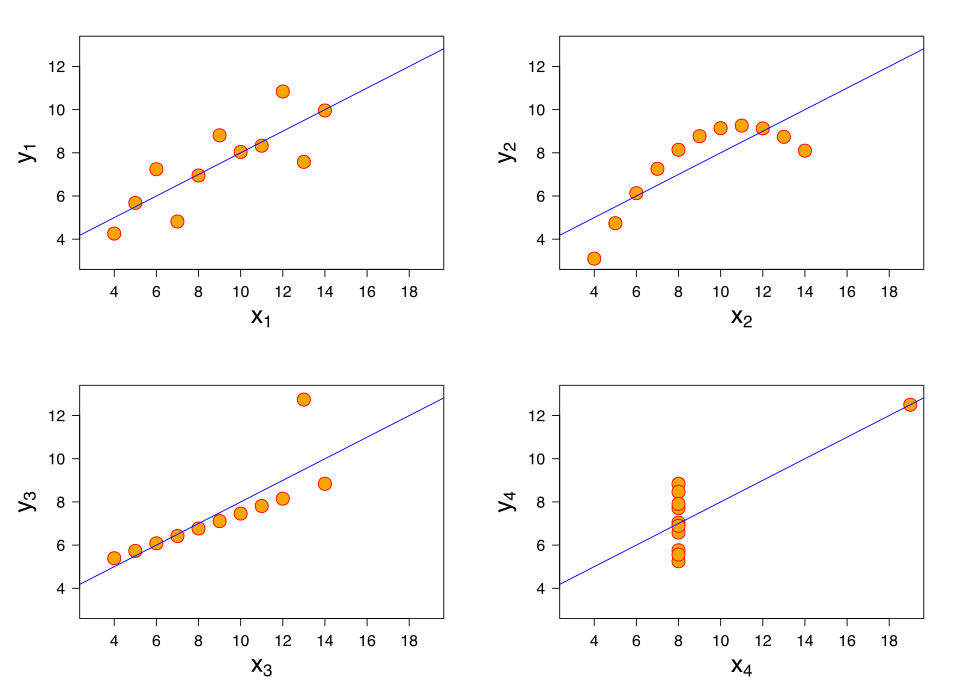
\includegraphics[width=0.7\textwidth]{Anscombe_quartet_3.svg.png}}
  \begin{itemize}
  \item Examples of the formula $y\approx \mu_y + \frac{\rho(x,y)}{\sigma^2_x}\left(x-\mu_x\right)$
  \item In the same way, we could predict $x[n+1]$ from $x[n]$
  \end{itemize}
\end{frame}


\begin{frame}
  \begin{columns}
    \begin{column}{0.5\textwidth}
      \begin{itemize}
      \item Each pixel in this image has positive covariance with its neighbors
      \item Each pixel is random, but generally similar to its neighbor
      \item You can predict a pixel by guessing that it will resemble its neighbor
      \end{itemize}
    \end{column}
    \begin{column}{0.5\textwidth}
      \centerline{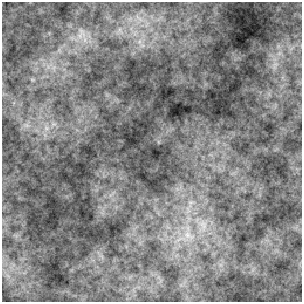
\includegraphics[width=\textwidth]{2D_pink_noise.png}}
    \end{column}
  \end{columns}
\end{frame}

\begin{frame}
  \frametitle{Autocorrelation and covariance}

  \begin{itemize}
  \item So what's the relationship?
  \item Autocorrelation:
  \begin{align*}
    \frac{r_x[n]}{N-n} =\frac{1}{N-n}\sum_{m=n}^{N-1} x[m]x[m-n] \approx E\left[x[m]x[m-n]\right]
  \end{align*}
  \item Covariance:
    \begin{align*}
      \rho_x[m,m-n]  = E\left[(x[m]-\mu_x[m])(x[m-n]-\mu_x[m-n])\right]
    \end{align*}
  \end{itemize}
\end{frame}

\begin{frame}
  \frametitle{Autocorrelation and covariance}

  Autocorrelation and covariance are the same thing ($\frac{1}{N-n}\sum_{m=n}^{N-1} x[m]x[m-n] \approx E\left[x[m]x[m-n]\right]\approx E\left[(x[m]-\mu_x[m])(x[m-n]-\mu_x[m-n])\right]$ if $x[n]$ is:
  \begin{enumerate}
  \item {\bf Wide-sense stationary:} $\rho_x[m,m-n]$ depends only on the delay ($n$),
    not the time at which you measure it ($m$)
  \item {\bf Zero-mean:} $\mu_x[m]=0$
  \end{enumerate}
  Under those circumstances,
  \begin{align*}
    \rho_x[m,m-n] &=E\left[x[m]x[m-n]\right]\\
    &\approx \frac{1}{N-n} r_x[n]
  \end{align*}
\end{frame}

\begin{frame}
  \frametitle{What kinds of signals are stationary?}

  Real signals are never stationary, but for denoising purposes, we can often
  break a signal down into
  \begin{align*}
    x[n] &= \mu_x[n] + v[n]
  \end{align*}
  \begin{itemize}
  \item Assume $\mu_x[n]$ is some expected signal that varies with time
  \item Assume $v[n]$ is a stationary zero-mean noise
  \end{itemize}
\end{frame}

%%%%%%%%%%%%%%%%%%%%%%%%%%%%%%%%%%%%%%%%%%%%%%%%%%%%%%%%%%%%%%%%%%%%%%%%%%%
\section[Convolution]{Autocorrelation and convolution}

\begin{frame}
  \frametitle{Autocorrelation is flipped convolution}

  Remember the formula for convolution:
  \begin{align*}
    x[n]\ast h[n] = \sum_{m=-\infty}^\infty x[m]h[n-m]
  \end{align*}
  Compare to the formula for autocorrelation:
  \begin{align*}
    r_x[n] = \sum_{m=-\infty}^\infty x[m]x[m-n]
  \end{align*}
  Lo and behold:
  \begin{align*}
    r_x[n] = x[n]\ast x[-n]
  \end{align*}
\end{frame}

\begin{frame}
  \frametitle{Autocorrelation is flipped convolution}

  \centerline{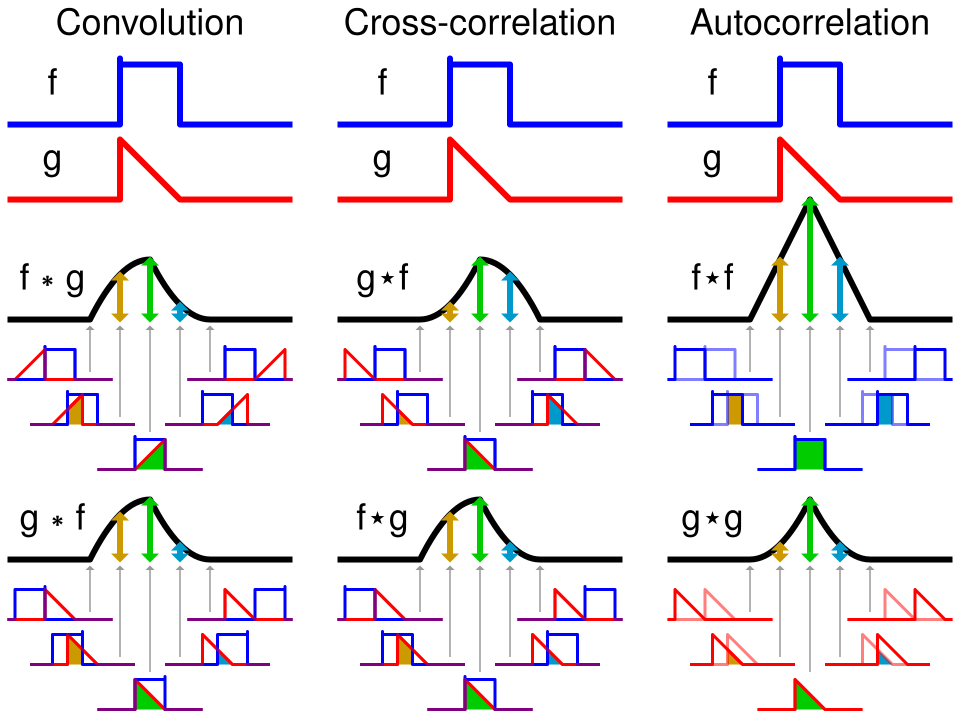
\includegraphics[width=\textwidth]{Comparison_convolution_correlation.svg.png}}
\end{frame}

\begin{frame}
  \frametitle{Try the quiz!}
  Go to the course web page and try the quiz!
\end{frame}

\begin{frame}
  \frametitle{Energy is $r_x[0]$}

  \begin{itemize}
  \item Energy is $r_x[0]$:
    \begin{align*}
      \mathcal{E}_x &= \sum_{m=-\infty}^\infty x^2[m] = r_x[0]
    \end{align*}
  \item Power = Variance = $\rho_x[0,0]$ = $\frac{1}{N}E\left[r_x[0]\right]$:
    \begin{align*}
      \sigma_x^2 &= E\left[(x-\mu_x)^2\right] = \frac{1}{N}E\left[r_x[0]\right]
    \end{align*}
  \end{itemize}
\end{frame}

\begin{frame}
  \frametitle{Autocorrelation is less than or equal to energy}

  \begin{align*}
    \sum_{m=n}^{N-1} x[m]x[m-n] &\le \sum_{m=0}^{N-1} x^2[m]
  \end{align*}
  And therefore
  \begin{align*}
    r_x[m] & \le r_x[0]
  \end{align*}

\end{frame}

%%%%%%%%%%%%%%%%%%%%%%%%%%%%%%%%%%%%%%%%%%%%%%%%%%%%%%%%%%%%%%%%%%%%%%%%%%%%%%
\section[Spectrum]{Autocorrelation and power spectrum}


\begin{frame}
  \frametitle{Fourier transform of time-flipped $x[n]$}

  What is the Fourier transform of $x[-n]$?
  \begin{align*}
    \mathcal{F}\left\{x[-n]\right\} &= \sum_{m=-\infty}^\infty x[-m]e^{-j\omega m}\\
    &= \sum_{m=-\infty}^\infty x[-m]e^{j(-\omega)m}\\
    &= X(-\omega)
  \end{align*}
  So the DTFT of $x[-n]$ is just $X(-\omega)$!  For real-valued
  $x[n]$, this is $X^*(\omega)$.
\end{frame}

\begin{frame}
  \frametitle{Fourier transform of the autocorrelation}

  What is the Fourier transform of $r_x[n]$?
  \begin{align*}
    \mathcal{F}\left\{r_x[n]\right\}
    &=\mathcal{F}\left\{x[n]\ast x[-n]\right\}\\
    &=\mathcal{F}\left\{x[n]\right\}\times\mathcal{F}\left\{\ast x[-n]\right\}\\
    &=X(\omega)X^*(\omega)\\
    &=|X(\omega)|^2
  \end{align*}
\end{frame}

\begin{frame}
  \frametitle{Power spectrum}

  \begin{itemize}
  \item The \textbf{power spectrum} is defined to be
    $E\left[|X(\omega)|^2\right]$.  Since the Fourier transform and
    expectation are both linear, we can swap their order, so that
    \begin{align*}
      E\left[|X(\omega)|^2\right] &=  E\left[\mathcal{F}\left\{r_x[n]\right\}\right]\\
      &=  \mathcal{F}\left\{E\left[r_x[n]\right]\right\}
    \end{align*}
  \item The \textbf{short-time power spectrum} (the one we'll deal
    with most often in this class) is just the DTFT of the
    autocorrelation of a short-time signal:
    \begin{align*}
      \mathcal{F}\left\{r_x[n]\right\}
      &=|X(\omega)|^2
    \end{align*}
  \end{itemize}
\end{frame}

%%%%%%%%%%%%%%%%%%%%%%%%%%%%%%%%%%%%%%%%%%%%%%%%%%%%%%%%%%%%%%%%%%%%%%%%%%%%%%
\section[White Noise]{Examples: white noise and pink noise}

\begin{frame}
  \frametitle{Example: White Noise}

  \begin{itemize}
  \item For example, \textbf{white noise} is a signal whose samples
    are completely uncorrelated with each other:
    \begin{align*}
      E\left[r_x[n]\right] &= E\left[x[m]x[m-n]\right]\\
      &= \delta[n]
    \end{align*}
  \item This is called white noise because its Fourier transform has
    equal energy at all frequencies, like white light:
    \begin{align*}
      E\left[|X(\omega)|^2\right] &=
      \mathcal{F}\left\{\delta[n]\right\}\\ &= 1
    \end{align*}
  \end{itemize}
\end{frame}

\begin{frame}
  \frametitle{Example: Pink Noise}
  \begin{itemize}
  \item \textbf{Pink Noise} is a signal whose samples have a small positive
    correlation with each other.  For example:
    \begin{align*}
      E\left[r_x[n]\right] &= \begin{cases}
        1 & n=0\\
        r/2 & |n|=1\\
        0 & |n|>1
      \end{cases}
    \end{align*}
  \item It's called \textbf{pink noise} because it has more energy at
    low frequencies, like red light:
    \begin{align*}
      E\left[|X(\omega)|^2\right] &=
      \mathcal{F}\left\{E\left[r_x[n]\right]\right\}\\
      &= 1+r\cos(\omega)\\
      &=\begin{cases}1+r & \omega=0\\
      1 &\omega=\frac{\pi}{2}\\
      1-r &\omega=\pi
      \end{cases}
    \end{align*}
  \end{itemize}
\end{frame}

\begin{frame}
  \frametitle{Spectrum of pink noise}
  \centerline{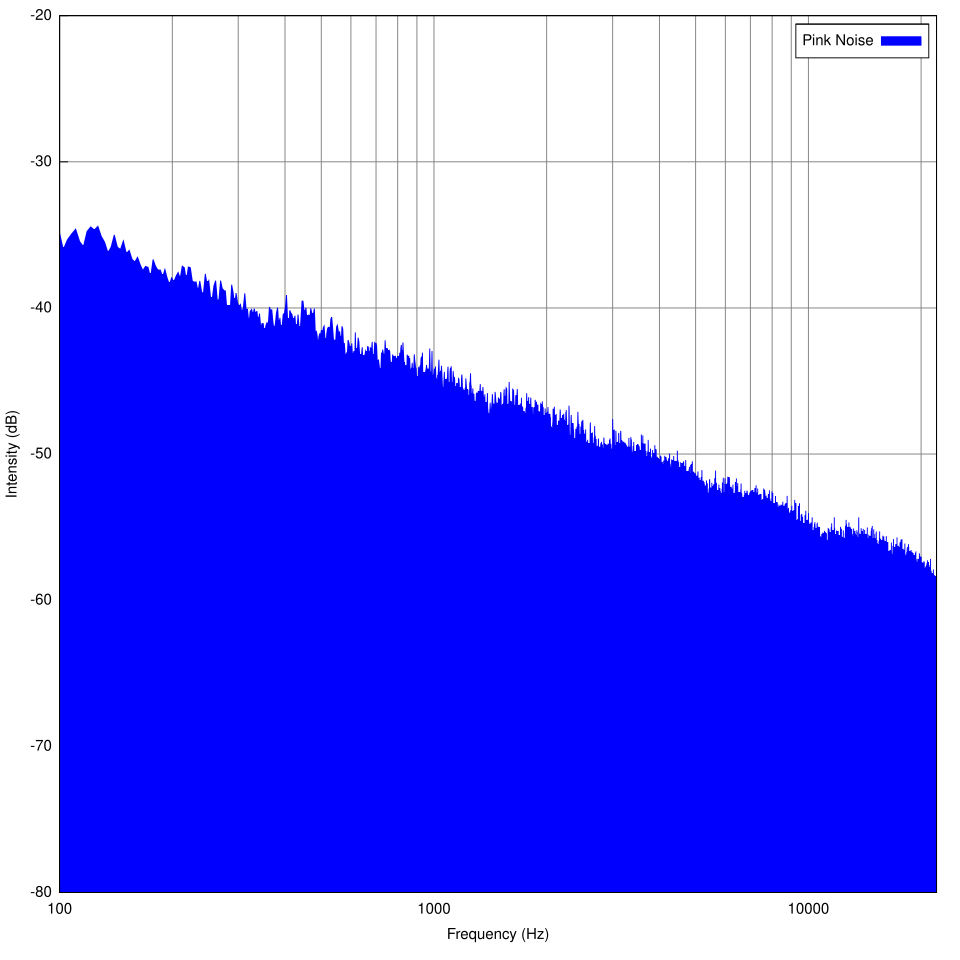
\includegraphics[width=\textwidth]{Pink_noise_spectrum.svg.png}}
\end{frame}

%%%%%%%%%%%%%%%%%%%%%%%%%%%%%%%%%%%%%%%%%%%%%%%%%%%%%%%%%%%%%%%%%%%%%%%%%%%%%%
\section{Summary}

\begin{frame}
  \frametitle{Summary}

  \begin{itemize}
  \item Autocorrelation:
    \begin{align*}
      r_x[n] = \sum_{m=-\infty}^\infty x[m]x[m-n]
    \end{align*}
  \item If the signal is stationary and zero-mean, then autocorrelation
    is a scaled estimate of covariance:
    \begin{align*}
      \rho_x[m,m-n] &=E\left[(x[m]-\mu_x[m])(x[m-n]-\mu_x[m-n])\right]
    \end{align*}
  \item Autocorrelation is flipped convolution:
    \begin{align*}
      r_x[n] = x[n]\ast x[-n]
    \end{align*}
  \item Power spectrum is the DTFT of convolution:
    \begin{align*}
      \mathcal{F}\left\{r_x[n]\right\}
      &=|X(\omega)|^2
    \end{align*}
  \end{itemize}
\end{frame}
    
\end{document}
